\documentclass[11pt,a4paper]{article}

\usepackage[margin=2.5cm]{geometry}
\usepackage{mathptmx}
\usepackage{caption}
\usepackage{float}
\captionsetup{font=small,labelfont=bf}
\setlength{\parskip}{4pt}

\usepackage[T1]{fontenc}
\usepackage{graphicx}
\usepackage{booktabs}
\usepackage{array}
\usepackage{amsmath}
\usepackage{url}
\usepackage[hidelinks,pdftitle={How Long Do Indian District-Court Cases Take? Predicting Disposal Within a Year at Filing},
  pdfauthor={Yashvanth S, Jeevanandham T, Nithillakrishi PY},
  pdfsubject={CS3006 Introduction to Data Science for Engineers, IIITDM Kancheepuram},
  pdfkeywords={Indian courts, eCourts, case duration, logistic regression},
  pdflang={en-GB}]{hyperref}

\graphicspath{{../../pipeline/reports/figures/}{../../pipeline/docs/screenshots/}}

\begin{document}

\title{How Long Do Indian District-Court Cases Take?\\
Predicting Disposal Within a Year at Filing}

\author{
\begin{tabular}{@{}c@{\hspace{3em}}c@{\hspace{3em}}c@{}}
Yashvanth S & Jeevanandham T & Nithillakrishi PY\\
CS24I1029 & CS24I1035 & CS24I1039
\end{tabular}\\[8pt]
CS3006 Introduction to Data Science for Engineers\\
IIITDM Kancheepuram}
\date{November 2026}

\maketitle

\begin{abstract}
Court cases in India often take years. We wanted to know which cases take long, and whether we can
tell this on the day a case is filed. We used public records of 80.9 million court cases from 2010
to 2018 and studied the 3.64 million cases from Tamil Nadu. We cleaned the data, fixed two problems
that would have made cases look faster than they are, and trained a model to answer one question:
will this case finish within a year? We tested it on 549,273 cases filed in 2017 that it had never
seen. It is right 80.9\% of the time, but most of that comes from easy cases. For real disputes it
is right 74.3\% of the time, while simply guessing ``no'' every time is right 72.0\% of the time. So
the type of case tells a lot, but on the first day we cannot say which dispute will be quick.
\end{abstract}

\noindent\textbf{Keywords:} Indian courts, eCourts, case duration, data cleaning, logistic regression

\section{Introduction}
Delays in Indian courts are well known, but people usually talk about total pending cases. We asked
a simpler question: \emph{if we only know what is written on the day a case is filed, can we say
whether it will finish within one year?} By ``finish'' we mean the case ended in that court, by a
judgment, dismissal, settlement or Lok Adalat. If a case was sent to another court, we do not count
that as finished.

This kind of answer can help a court plan its work, for example to estimate how many of this year's
new cases will still be pending next year. It is not meant to predict any one person's case. We
set two rules for ourselves: the model can only use information known on the filing day, and it
must do better than a simple table of past averages. If it cannot beat that table, there is no
point in using it.

\section{Data}
We used data from Development Data Lab \cite{ddl}, who collected and anonymised records from the
government's eCourts website. It has 80,935,944 cases filed in district courts across India from
2010 to 2018, shared under the ODbL v1.0 licence \cite{odbl}. Each row is one case. It tells us the
district and court, the type of case, how it ended, and five dates: filing, decision, first
hearing, last hearing and next hearing. A second file gives the law and section the case was filed
under. Names of people are not included.

We focused on Tamil Nadu (3,640,055 cases), since our institute is here. We used the all-India data
only to find out when the data was collected. The data is only available as one very large
download, so we wrote a script that reads it as it downloads, keeps only the files we need, and
checks that each file arrived correctly.

\section{Preparing the Data}

\subsection{Cleaning}
Most fields were typed by hand by court staff, so the same thing is written in many ways.
Table~\ref{tab:clean} shows the main fixes. When a value was clearly wrong, such as a date in the
year 7201, we removed it and counted how many there were, instead of guessing. We also removed
23,497 cases that were ``decided before they were filed''. Cases sent to another court (14\%) are
marked as ``moved'', not finished. We wrote 142 tests to check that the cleaning rules work on real
examples from the data.

\begin{table}[H]
\caption{Main cleaning steps (Tamil Nadu)}
\label{tab:clean}
\centering\small
\begin{tabular}{@{}>{\raggedright\arraybackslash}p{0.45\textwidth}>{\raggedright\arraybackslash}p{0.40\textwidth}@{}}
\toprule
Problem & What we did \\
\midrule
Law names written 29,857 different ways & Grouped into 54 laws \\
Section numbers as free text (``138r/w142'') & Read out the main section \\
116 spellings of court names & Grouped into 14 court types \\
Impossible dates (year 0001, 7201) & Removed and counted \\
52 different ``how it ended'' codes & Grouped; transfers marked ``moved'' \\
\bottomrule
\end{tabular}
\end{table}

\subsection{When was the data collected?}
If a case has no decision date, we only know it was still pending on the day the data was
collected. But the data does not tell us that day. We found it from the number of decisions per
month (Fig.~\ref{fig:cliff}). Across India there were about one million decisions every month in
2018, and then the count suddenly drops in January and February 2019. That drop is when the data
was collected. We worked out this date for each district separately.

\begin{figure}[H]
\centering
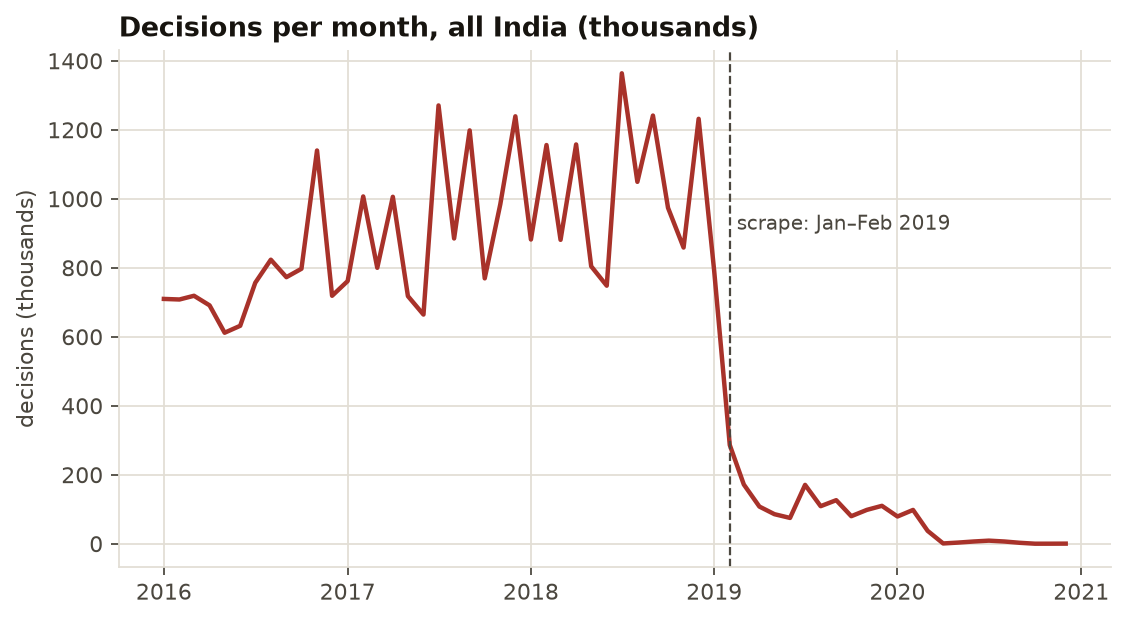
\includegraphics[width=0.62\textwidth]{eda_scrape_cliff.png}
\caption{Decisions recorded per month across India. The sudden drop in early 2019 shows when the
data was collected.}
\label{fig:cliff}
\end{figure}

\subsection{The early years are incomplete}
The same 592 courts in Tamil Nadu have 170,958 cases filed in 2010 but 622,473 filed in 2018.
Courts did not get 3.6 times busier. Cases that finished quickly before the courts started using
computers were mostly never entered, so the old years look much slower than they really were. For
this reason we only used cases filed from 2015 to 2017.

\subsection{Labels}
For each case we want a yes or no answer: did it finish within 365 days? We only give this answer
if the case was filed at least one year before the data was collected, so that every case had a
full year to finish. Our first attempt skipped this rule, and it said 93\% of 2018 cases finished
within a year, which was clearly wrong. After the fix, the share of cases finishing within a year
is 35.9\% for 2015 (405,062 cases), 43.5\% for 2016 (445,639) and 49.5\% for 2017 (549,273).

\section{What the Data Shows}

\paragraph*{A misleading average} If we take only the cases that have finished, the typical
(median) time falls from 1,366 days for 2010 cases to just 17 days for 2017 cases. This is not
because courts became faster. It is because many 2017 cases had not finished yet, so only the
quick ones were counted. A Kaplan--Meier estimate \cite{km}, which also counts the cases that are
still pending, shows a much smaller fall (Fig.~\ref{fig:median}). By this method, a typical case
filed between 2015 and 2018 takes 532 days.

\begin{figure}[H]
\centering
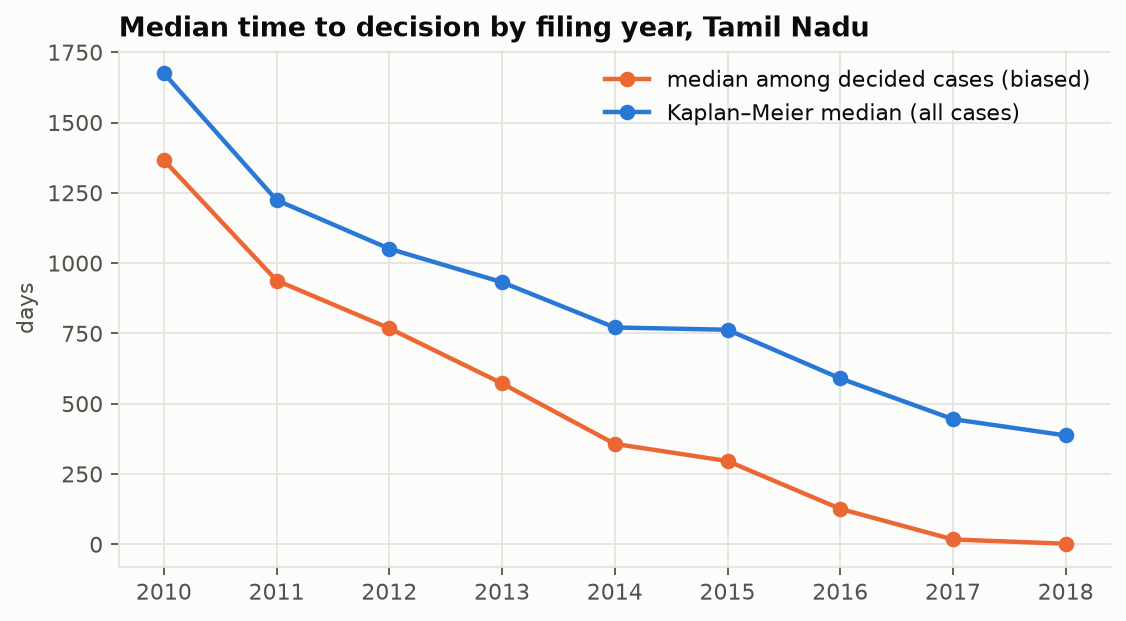
\includegraphics[width=0.6\textwidth]{eda_median_trap.png}
\caption{Typical (median) time to a decision by filing year in Tamil Nadu. Black: only finished
cases. Red: Kaplan--Meier, which also counts pending cases.}
\label{fig:median}
\end{figure}

\paragraph*{Type of case matters most} 98\% of bail-type petitions and 80\% of petty-offence cases
finish within a year, but only 28\% of civil suits and 12\% of accident claims do
(Fig.~\ref{fig:open}). Between districts the share goes from 19\% to 74\%. We tried grouping
districts with k-means, but they did not form clear groups.

\begin{figure}[H]
\centering
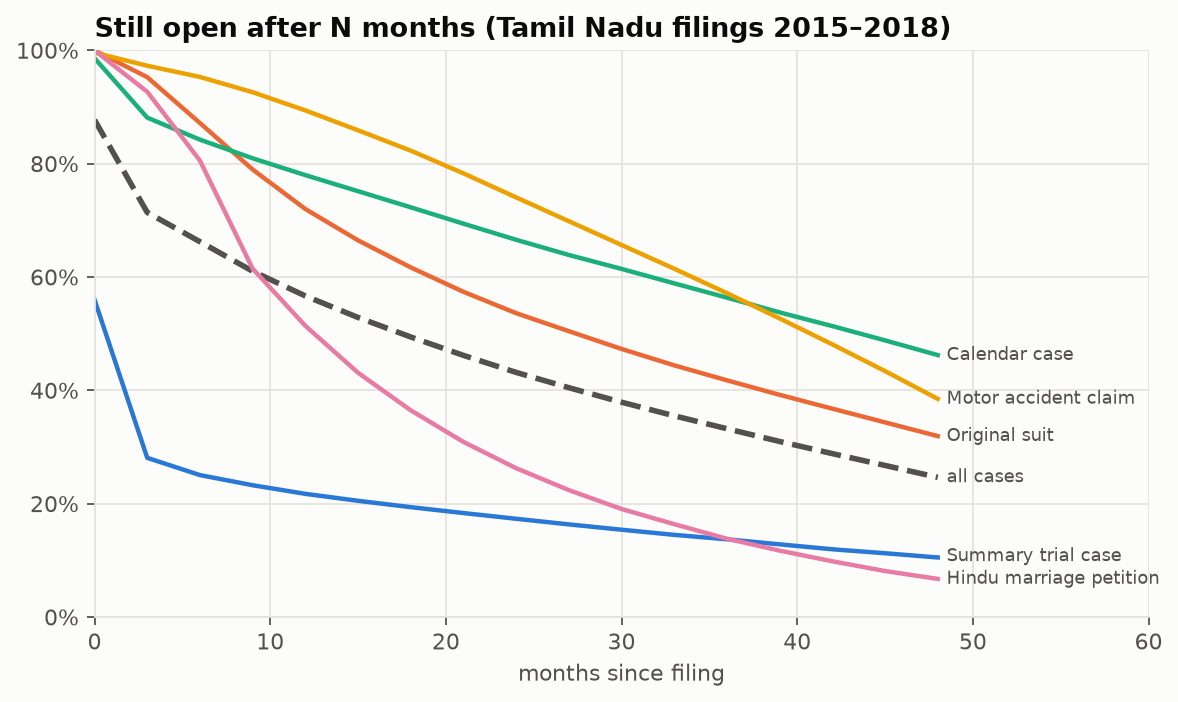
\includegraphics[width=0.62\textwidth]{survival_still_open.png}
\caption{Share of Tamil Nadu cases (filed 2015--2018) still pending after a given number of months,
for each type of case.}
\label{fig:open}
\end{figure}

\paragraph*{Where the time goes} We call every case except petty-offence cases and bail-type
petitions a \emph{real dispute}. A real dispute waits about 40 days for its first hearing, and then
goes on for about 808 more days. So 95\% of the time is spent after the first hearing.

\section{Method}

\paragraph*{What the model sees} Twelve facts known on the filing day: the district, the court,
the type of case, the month, the law and section, whether the offence is bailable, whether it is
criminal or civil, the number of sections charged, how many cases are already pending in those
courts, how many cases they finished last year, and how many cases of this type were filed there
last year. We did not use hearing dates, because they happen after filing. We did not use gender,
because a public tool should not judge a case by the gender of the people in it.

\paragraph*{How we tested} We trained on 2015 cases and used 2016 cases to choose the best model.
Then we trained that model again on 2015 and 2016 (850,701 cases) and tested it only once, on 2017
cases (549,273). The 2017 cases were never used before the final test.

\paragraph*{Models} We compared three simple ``past average'' tables (overall, by case type, and by
case type and district) with three models from scikit-learn \cite{sklearn}: logistic regression, a
linear SVM and a random forest \cite{rf}. We measured accuracy, AUC \cite{auc} (how well the model
puts quick cases above slow ones; 0.5 is guessing, 1.0 is perfect) and the Brier score \cite{brier}
(how close the predicted chances are to what happened; lower is better). Logistic regression did
best on the 2016 cases, so that is the model we use. Saved, it is only 6\,kB.

\section{Results}
Table~\ref{tab:results} shows the 2017 test. Our model is better than the best past-average table
(AUC 0.873 against 0.844, Brier score 0.138 against 0.163). The SVM and random forest give almost
the same numbers, so a more complex model did not help. The model's chances can also be trusted:
when it says 55\%, the case finishes within a year 56\% of the time, and when it says 85\%, it
happens 87\% of the time (Fig.~\ref{fig:cal}).

\begin{table}[H]
\caption{Test on 2017 cases (549,273 cases)}
\label{tab:results}
\centering\small
\begin{tabular}{@{}lccc@{}}
\toprule
Method & AUC & Brier & Accuracy \\
\midrule
Overall average & 0.500 & 0.259 & 50.5\% \\
Average by case type & 0.828 & 0.163 & 78.0\% \\
Average by case type and district & 0.844 & 0.163 & 75.9\% \\
Logistic regression (our model) & \textbf{0.873} & \textbf{0.138} & \textbf{80.9\%} \\
Linear SVM & 0.873 & 0.137 & 81.1\% \\
Random forest & 0.874 & 0.138 & 80.7\% \\
\bottomrule
\end{tabular}
\end{table}

\begin{figure}[H]
\centering
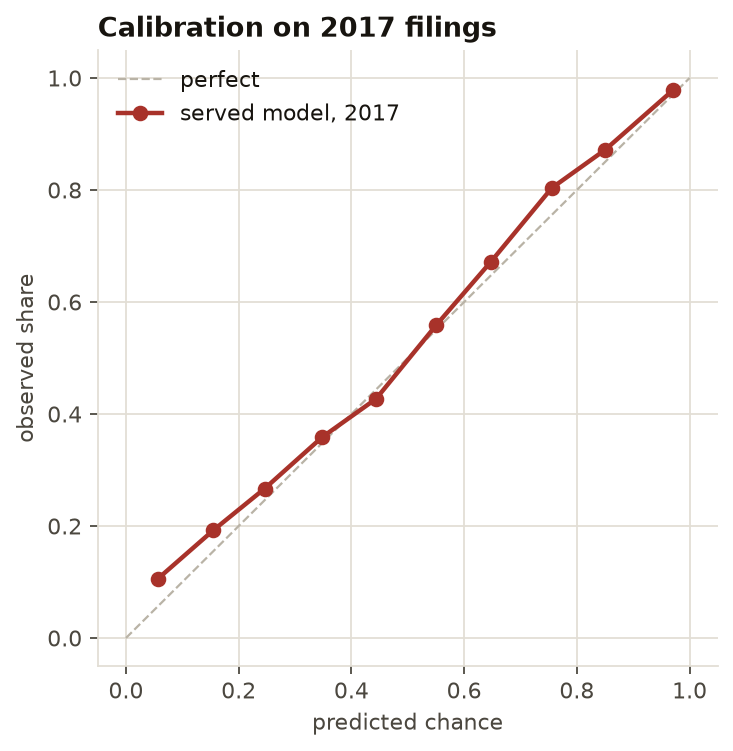
\includegraphics[width=0.42\textwidth]{model_calibration.png}
\caption{Predicted chance against what really happened, 2017 cases. Points close to the diagonal
mean the predicted chances are correct.}
\label{fig:cal}
\end{figure}

However, 80.9\% accuracy is less impressive than it sounds. Petty-offence cases and bail-type
petitions almost always finish within a year, and the model only has to recognise them.
Table~\ref{tab:split} splits the test cases into easy cases and real disputes. \textbf{For real
disputes the model is right 74.3\% of the time, while always saying ``no'' is right 72.0\% of the
time.} Models trained only on real disputes did not do better either. This means the problem is
not the algorithm: the information available on the filing day is simply not enough to tell which
dispute will be quick.

\begin{table}[H]
\caption{Model accuracy against always guessing the most common answer, 2017}
\label{tab:split}
\centering\small
\begin{tabular}{@{}lrccc@{}}
\toprule
Cases & Number & Model & Guessing & AUC \\
\midrule
All & 549,273 & 80.9\% & 50.5\% & 0.873 \\
Easy cases & 196,105 & 92.6\% & 88.1\% & 0.903 \\
Real disputes & 353,168 & 74.3\% & 72.0\% & 0.706 \\
\bottomrule
\end{tabular}
\end{table}

\section{Website}
We put the model online at \url{https://otlr.vercel.app/model}. A small Python server (FastAPI)
runs the model, and the website (Next.js) lets anyone pick a case, press Analyze and see the
chance of it finishing within a year, how much to trust that number, and which facts pushed it up
or down. The site also shows our data analysis and every step of the pipeline with its code. A
test checks that the website gives exactly the same answer as our pipeline.

\section{Limitations}
The high overall accuracy mostly comes from easy cases. The data covers only Tamil Nadu cases filed
from 2015 to 2017, and courts may have changed since then. The collection date is our estimate,
not a recorded fact, and some cases that look pending may simply never have been updated. The
model is meant for planning, not legal advice, and should not be used to make decisions about any
one person's case.

\section{Conclusion}
We built a complete pipeline: downloading 80.9 million records, cleaning them, fixing the
collection date and the missing early cases, exploring the data, building and testing a model, and
putting it on a website. On the filing day we can tell which \emph{type} of case will be quick, but
not which dispute will be (74.3\% against 72.0\% for guessing). Since 95\% of a dispute's time is
spent after the first hearing, delays seem to depend mainly on what happens once the case starts.
In future, a model that updates its prediction after each hearing could do much better.

\section*{Contributions}
All three of us contributed equally. Yashvanth S built and tested the models, the model server
and the deployment. Jeevanandham T handled the data download, the cleaning rules and their tests,
and the labels (collection date, moved cases, missing early cases). Nithillakrishi PY did the data
analysis, the survival curves and clustering, the notebooks and figures, and the website pages.

\section*{Data and Code}
Contains data from Development Data Lab's judicial data, ODbL v1.0. All code, notebooks and
results: \url{https://github.com/YashvanthSankar/idse-course-project} (folder \texttt{pipeline/}).

\begin{thebibliography}{7}\small
\bibitem{ddl} Development Data Lab, ``Judicial data: Indian district court records (eCourts),
2010--2018.'' [Online]. Available: \url{https://www.devdatalab.org/judicial-data}
\bibitem{odbl} Open Data Commons, ``Open Database License (ODbL) v1.0.'' [Online]. Available:
\url{https://opendatacommons.org/licenses/odbl/1-0/}
\bibitem{km} E.~L. Kaplan and P.~Meier, ``Nonparametric estimation from incomplete observations,''
\emph{J. Amer. Statist. Assoc.}, vol.~53, no.~282, pp.~457--481, 1958.
\bibitem{auc} J.~A. Hanley and B.~J. McNeil, ``The meaning and use of the area under a receiver
operating characteristic (ROC) curve,'' \emph{Radiology}, vol.~143, no.~1, pp.~29--36, 1982.
\bibitem{brier} G.~W. Brier, ``Verification of forecasts expressed in terms of probability,''
\emph{Monthly Weather Rev.}, vol.~78, no.~1, pp.~1--3, 1950.
\bibitem{rf} L.~Breiman, ``Random forests,'' \emph{Mach. Learn.}, vol.~45, no.~1, pp.~5--32, 2001.
\bibitem{sklearn} F.~Pedregosa \emph{et al.}, ``Scikit-learn: Machine learning in Python,''
\emph{J. Mach. Learn. Res.}, vol.~12, pp.~2825--2830, 2011.
\end{thebibliography}

\end{document}
